\documentclass[a4paper,12pt]{article}

\usepackage{comment}
\usepackage{supertabular}
\usepackage{graphics}
\usepackage{color,soul}
\usepackage{booktabs}
\usepackage{paralist}
\usepackage{algorithmicx}
\usepackage{algorithm}
\usepackage[noend]{algpseudocode}
\usepackage{booktabs}
\usepackage{hvfloat}
\usepackage{comment}
\usepackage{chngpage}
\usepackage{url}
\usepackage[utf8]{inputenc}
\usepackage[table,dvipsnames]{xcolor}
\usepackage[a4paper,pdftex,hmargin=0.75in,vmargin={1.1in,0.6in},head=75pt,foot=45pt, left=2.5cm, right=2.5cm, includefoot, footskip=60pt]{geometry}
\usepackage{lipsum}
\usepackage{afterpage}
\usepackage{xcolor}
\usepackage{tabularx}
\usepackage{wallpaper}
\usepackage{adjustbox}
\usepackage[normalem]{ulem}
\useunder{\uline}{\ul}{}
\usepackage{rotating}
\usepackage{parskip}
\usepackage{listings}
\lstset{language=C,breaklines=true}
\usepackage[english]{babel}
\usepackage{amsmath}
\usepackage{amsfonts}
\usepackage{amssymb}
\usepackage[justification=centering]{caption}
\usepackage{fontenc}
\usepackage{multicol}
\usepackage{multirow}
\usepackage{array}
\usepackage{relsize}
\usepackage{subcaption}
\usepackage{caption}
\usepackage[colorlinks=true,pdfusetitle]{hyperref}
\usepackage{tcolorbox}
\usepackage{lscape}
\usepackage{lastpage}
\usepackage{acro}
\setlength{\headsep}{1.5cm}
\usepackage[toc,page]{appendix}
\usepackage[nottoc]{tocbibind} % for show references in toc
\usepackage{pgfgantt}
\frenchspacing
%\usepackage{svg}
%\usepackage{showframe}% for show page layout

%%%%%%%%%%%%%%
% Set by Oscar
%%%%%%%%%%%%%%
\usepackage{microtype}
\usepackage[newfloat,draft=false]{minted}

\colorlet{punct}{red!60!black}
\definecolor{background}{HTML}{EEEEEE}
\definecolor{delim}{RGB}{20,105,176}
\colorlet{numb}{magenta!60!black}
\lstdefinelanguage{json}{
    basicstyle=\normalfont\ttfamily,
    numbers=left,
    numberstyle=\scriptsize,
    stepnumber=1,
    numbersep=8pt,
    showstringspaces=false,
    breaklines=true,
    frame=lines,
    backgroundcolor=\color{background},
    literate=
     *{0}{{{\color{numb}0}}}{1}
      {1}{{{\color{numb}1}}}{1}
      {2}{{{\color{numb}2}}}{1}
      {3}{{{\color{numb}3}}}{1}
      {4}{{{\color{numb}4}}}{1}
      {5}{{{\color{numb}5}}}{1}
      {6}{{{\color{numb}6}}}{1}
      {7}{{{\color{numb}7}}}{1}
      {8}{{{\color{numb}8}}}{1}
      {9}{{{\color{numb}9}}}{1}
      {:}{{{\color{punct}{:}}}}{1}
      {,}{{{\color{punct}{,}}}}{1}
      {\{}{{{\color{delim}{\{}}}}{1}
      {\}}{{{\color{delim}{\}}}}}{1}
      {[}{{{\color{delim}{[}}}}{1}
      {]}{{{\color{delim}{]}}}}{1},
}

%RBG FFD33E / C95D40
\definecolor{upcorange}{HTML}{FFD33E}
\hypersetup{linkcolor=blue}

% probably a good idea for the nomenclature entries:
\acsetup{first-style=short}

%%%% PAGE STYLE %%%%%
\usepackage{fancyhdr}
\pagestyle{fancy}
\fancyhf{}
\lhead{
\includegraphics[height=1.2cm]{img/logos/upclogo.png}}
\rhead{
\includegraphics[height=1.2cm]{img/logos/logo_telecos.png}}
\rfoot{\thepage{}}

\renewcommand{\footrulewidth}{0.4pt}
%\futurelet\TMPfootrule\def\footrule{{\color{upcorange}\TMPfootrule}}
\futurelet\TMPfootrule\def\footrule{{\color{gray!80}\TMPfootrule}}
\renewcommand{\headrulewidth}{0.4pt}
\renewcommand{\headrule}{\hbox to\headwidth{%
%\color{upcorange}\leaders\hrule height \headrulewidth\hfill}}
\color{gray!80}\leaders\hrule height \headrulewidth\hfill}}
%\renewcommand*\ShowFrameColor{\color{red}}

%%% TEMPORAL
%% for 1.5 line spacing
\usepackage{setspace}
\onehalfspacing


\begin{document}

%%% COVER %%%

\fancypagestyle{alim}{\fancyhf{}\renewcommand{\headrulewidth}{0pt}
\cfoot{
\includegraphics[height=2.2cm]{img/logos/logo_telecos.png}}
}
\thispagestyle{empty}
\begin{center}
{\sffamily 
\resizebox{0.8\textwidth}{!}{
\includegraphics{img/logos/upc_completo+telecos.png}}\\
\vspace{1cm}
{\Huge Thesis title}\\
\vspace{0.5cm}
{\color{black}\hrule height 1pt}
\vspace{1cm}
{\large{Degreeee Thesis / Treball Fi de Grau / Trabajo Fin de Grado\\
submitted to the Faculty of the / realitzada a l' / realizada en la \\
Escola T\`ecnica d'Enginyeria de Telecomunicaci\'o de Barcelona \\
Universitat Polit\`ecnica de Catalunya \\
by / per / por \\
\vspace{0.5cm}
%{\Huge{Student name}}
Student name}}

\vspace{1.5cm}

{In partial fulfillment / En compliment parcial / En cumplimiento parcial\\
of the requirements for the degree in / dels requisits per al Grau en / de los requisitos para el Grado en \\
\textit{(Write the name of your Degree)} \textbf{ENGINEERING}}

\vspace{2cm}

{{Advisor / Director/ Directora: name of the advisor\\}}
{{Barcelona, Date XXXXX}}

\vspace{2cm}

{\color{red} \textbf{Note:} Please note this frontpage is provided in the three official languages. Please select one and delete this note as well.}
\thispagestyle{alim}
}

\end{center}

%%% INDEX %%%
\newpage
\tableofcontents

%%% LISTS %%%
\newpage
\listoffigures
\lstlistoflistings
\listoftables

\newpage

%%% ABSTRACT %%%
\newpage
\section*{Abstract}

{Every copy of the thesis must have an abstract. An abstract must provide a concise summary of the thesis. In style, the
abstract should be a miniature version of the thesis: short introduction, a summary of the results, conclusions or main
arguments presented in the thesis. The abstract may not exceed 150 words for a Degree’s thesis.}

\newpage
\section*{Revision history and approval record}
\begin{center}
\tablefirsthead{}
\tablehead{}
\tabletail{}
\tablelasttail{}
\begin{supertabular}{|m{1.908cm}|m{2.398cm}|m{11.489cm}|}
\hline
\selectlanguage{english} \foreignlanguage{english}{\textbf{Revision}} &
\selectlanguage{english} \foreignlanguage{english}{\textbf{Date}} &
\selectlanguage{english} \foreignlanguage{english}{\textbf{Purpose}}\\\hline
\selectlanguage{english} \foreignlanguage{english}{0} &
\selectlanguage{english} \foreignlanguage{english}{01/06/2021} &
\selectlanguage{english} \foreignlanguage{english}{Document \ creation}\\\hline
\selectlanguage{english} \foreignlanguage{english}{1} &
\selectlanguage{english} \foreignlanguage{english}{dd/mm/yyyy} &
\selectlanguage{english} \foreignlanguage{english}{Document \ revision}\\\hline
~
 &
~
 &
~
\\\hline
~
 &
~
 &
~
\\\hline
~
 &
~
 &
~
\\\hline
\end{supertabular}
\end{center}

\bigskip

\selectlanguage{english}
DOCUMENT DISTRIBUTION LIST

\begin{center}
\tablefirsthead{}
\tablehead{}
\tabletail{}
\tablelasttail{}
\begin{supertabular}{|m{8.205cm}|m{7.589cm}|}
\hline
\selectlanguage{english} \foreignlanguage{english}{\textbf{\ Name}} &
\selectlanguage{english} \foreignlanguage{english}{\textbf{\ e-mail}}\\\hline
\selectlanguage{english} \foreignlanguage{english}{Òscar Pérez Castillo} &
~ \href{mailto:oscar.pz.castillo@gmail.com}{oscar.pz.castillo@gmail.com}
\\\hline
\selectlanguage{english} \foreignlanguage{english}{Jose Luis Muñoz Tapia} &
~
\\\hline
\selectlanguage{english} \foreignlanguage{english}{Rafael Genés Duran} &
~
\\\hline
~
 &
~
\\\hline
~
 &
~
\\\hline
~
 &
~
\\\hline
\end{supertabular}
\end{center}

\bigskip

\begin{center}
\tablefirsthead{}
\tablehead{}
\tabletail{}
\tablelasttail{}
\begin{supertabular}{|m{1.925cm}|m{6.1990004cm}|m{1.901cm}|m{5.6140003cm}|}
\hline
\multicolumn{2}{|m{8.324cm}|}{ Written by:} &
\multicolumn{2}{m{7.715cm}|}{Reviewed and approved by:}\\
\hline
\selectlanguage{english} Date &
\selectlanguage{english} dd/mm/yyyy &
\selectlanguage{english} Date &
\selectlanguage{english} dd/mm/yyyy\\\hline
\selectlanguage{english} Name &
\selectlanguage{english} Xxxxxxx yyyyyyy &
\selectlanguage{english} Name &
\selectlanguage{english} \foreignlanguage{english}{Zzzzzzz \ Wwwwwww}\\\hline
\selectlanguage{english} Position &
\selectlanguage{english} \foreignlanguage{english}{Project Author } &
\selectlanguage{english} \foreignlanguage{english}{Position} &
\selectlanguage{english} \foreignlanguage{english}{Project Supervisor}\\\hline
\end{supertabular}
\end{center}


\newpage

\clearpage\section{Introduction}

{An Introduction that clearly states the rationale of the thesis that includes:}

\begin{enumerate}
\item {Statement of purpose (objectives).}
\item {Requirements and specifications.}
\item {Methods and procedures, citing if this work is a continuation of another project or it uses applications, algorithms,
software or hardware previously developed by other authors.}
\item {Work plan with tasks, milestones and a Gantt diagram.}

\item {Description of the deviations from the initial plan and incidences that may have occurred. }
\end{enumerate}

\bigskip

{The minimum chapters that this thesis document should have are described below, nevertheless they can have different
names and more chapters can be added.}


\bigskip

\subsection{Gantt Diagram}
\label{ssec:gantt}
\begin{figure}[H]
    \centering
    %\includegraphics[width=13cm]{img/diagram_gantt.png}
    \begin{ganttchart}[y unit title=0.4cm,
y unit chart=0.5cm,
vgrid,hgrid,
title height=1,
%today=25,%
%today offset=.5,%
%today label=Now,%
%bar/.style={draw,fill=cyan},
bar incomplete/.append style={fill=yellow!50},
bar height=0.7]{1}{24}

 % dies
 \gantttitle{Phases of the Project}{24} \\
 \gantttitle{2021}{24} \\
 \gantttitle{Feb}{4}
 \gantttitle{Mar}{5}
 \gantttitle{April}{5}
 \gantttitle{May}{5}
 \gantttitle{Jun}{5} \\
 
 % caixes elem0 .. elem9 
 % INTRODUCTION
 \ganttgroup[inline=false]{Introduction}{1}{2}\\
 \ganttbar[progress=100,bar/.style={draw,fill=cyan}]{Learn Javascript}{1}{1} \\
 \ganttbar[progress=100,bar/.style={draw,fill=cyan}]{Learn about containers}{2}{2} \\

 % LXCE
 \ganttgroup[inline=false]{lxce}{3}{16}\\
 \ganttbar[progress=100,bar/.style={draw,fill=red}]{v0.1}{3}{5} \\
 \ganttbar[progress=100,bar/.style={draw,fill=red}]{v0.2}{6}{8} \\
 \ganttbar[progress=100,bar/.style={draw,fill=red}]{v0.3}{9}{16} \\

 % LXCE-ADMIN
 \ganttgroup[inline=false]{lxce-admin}{14}{16}\\
 \ganttbar[progress=100,bar/.style={draw,fill=white}]{v0.1}{14}{16} \\

 % WEB ADMIN
 \ganttgroup[inline=false]{lxce-admin}{17}{20}\\
 \ganttbar[progress=90,bar/.style={draw,fill=black}]{Learn React/redux}{17}{19} \\
 \ganttbar[progress=10,bar/.style={draw,fill=black}]{Implement application}{20}{20} \\

 % relations
\ganttlink{elem2}{elem4}
\ganttlink{elem8}{elem10}


\end{ganttchart}

    \caption[Project's Gantt diagram]{\footnotesize{Gantt diagram of the project}}
    \label{fig:gantt}
    For more information read the manual \cite{skalagantt} of Skala.
\end{figure}

\bigskip

\subsection{Topic}


%%% StateOfTheArt %%%
\clearpage\section{State of the art of the technology used or applied in this thesis:}

{A backgroundadajdasajdaskdasdsadsa, comprehensive review of the literature is required. This is known as the Review of Literature and should
include relevant, recent research that has been done on the subject matter.}

\subsection{Topic}

Here you have a couple of references about LaTeX ~\cite{latexcompanion} and electrodynamics \cite{einstein}.

\bigskip

\subsection{Topic}

%%% METHODOLOGY %%%
%\clearpage\section{Methodology / project development: }

%{The Methodology is included in this chapter and should include all relevant %methods that were utilized as well as
%research methods and measurements, software and hardware development, ...}

%%% RESULTS: SECTIONS %%%

%%% SECTION3 %%%
\newpage
%\vspace*{2cm}
\section{Section 3}
\label{sec:sec3}

\lipsum[4]  \lipsum[5]
\lipsum[6]  \lipsum[7]

\subsection{Subsection}
\label{sec:subsec3.1}
The book \cite{latexcompanion} \lipsum[15]

\begin{algorithm}
\caption{Temperature-Distributed algorithm}\label{alg:tempdistrib}
\begin{algorithmic}[1]
\Procedure{Temp-Spread}{$GN_i, HN_j, temperatures$}\Comment{Lowest temperature priority}
\State $temperature\_list\gets short(temperatures)$
\State $max_temperature\gets max(temperature_list)$
\State $ThresHold\gets 0.5$
\State $temperature\_impact \gets 0.2$
\For{$GN_i$ in $i=1,8$}\Comment{Iterate every hardware node on the given GN}
\State $it\_temperature \gets temperature\_list(GN_i)$
\State $temp\_weight \gets \frac{max\_temperature-it\_temperature}{max\_temperature}*temperature\_impact$
\State $\omega(Master-GN_i) \gets ThresHold*temp\_weight$
\For{$HN_j$ in $j=1,n$}
\If{$available\_accel_{i,j} > busy\_accel_{i,j}$}
    \State $policy_\omega = \frac{Available HW}{Total HW}*ThresHold$
    \State $\omega(GN_i-HN_{i,j}) \gets ThresHold+policy_\omega$
\Else
    \State $\omega(GN_i - HN_{i,j}) \gets 1$
\EndIf

\EndFor
\EndFor
\State $node \gets find\_djistra\_shortest\_path(Master\_Node, aux\_node)$
\State \textbf{$return node$} $b$\Comment{The gcd is b}
\EndProcedure
\end{algorithmic}
\end{algorithm}

%%% SECTION4 %%%
\clearpage
%\vspace*{2cm}
\section{Section 4}
\label{sec:sect4}
\lipsum[8]
\subsection{Subsection 4.1}
\label{subsec:subsec4.1}
\lipsum[8]
Read de book \cite{einstein} of Einstein.

\begin{figure}[H]
\label{fig:prototype1}
\centering
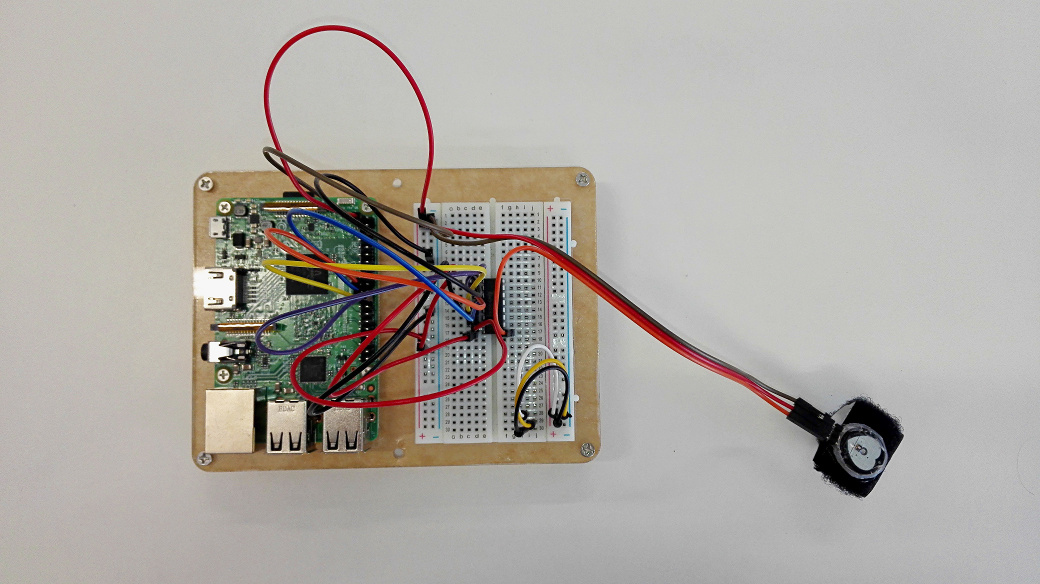
\includegraphics[width=10cm]{img/Chapter4/prototype1_edited.jpg}
\caption[Prototype setup]{\footnotesize{Prototype setup.}}
\end{figure}

\lipsum[14]

\subsection{Subsection 4.2}
\label{subsec:subsec4.2}

\begin{table}[H]
\centering
\caption[This is the caption]{ \footnotesize This is the other caption. Since the trial size of the experiments showed is one second, the number of \textit{Target} and \textit{Impostor} data corresponds to number of trials or seconds}
\label{tab:data_partition}
\footnotesize{
\begin{tabular}{@{}llcccc@{}}
\toprule
\textbf{Dataset}         & \multicolumn{1}{c}{\textbf{Label}} & \textbf{Train} & \textbf{Validation} & \textbf{Develop} & \textbf{Test} \\ \midrule
\midrule
\multirow{3}{*}{First} & Target   & $135$ & $45$  & $30$  & $30$  \\
                         & Impostor & $5,220$    & $1,740$ & $1,890$   & $2,880$    \\
\cmidrule(lr){3-5} \cmidrule(l){6-6}
                         & \#Subjects          & \multicolumn{3}{c}{$31$} & $12$ \\
\midrule
\multirow{3}{*}{Second}  & Target   & $144$ & $80$  & $48$  & $48$  \\
                         & Impostor & $2,014$    & $1,119$    & $1,343$    & $1,545$ \\
\cmidrule(lr){3-5} \cmidrule(l){6-6}
                         & \#Subjects   & \multicolumn{3}{c}{$15$} & $5$ \\ 
\bottomrule
\end{tabular}
}
\end{table}


%%% SECTION5 %%%
\newpage
%\vspace*{2cm}
\section{Section 5}
\label{sec:sect5}
\lipsum[4]

\subsection{Overview}
\label{subsec:sect5Overview}
\lipsum[10]
Visite the Knuth repository \cite{knuthwebsite}.

%%% TESTING %%%
\clearpage
%\vspace*{2cm}
\section{Experiments and results}
\label{sec:tests}
\lipsum[9]

%%% BUDGET %%%
\clearpage
\section{Budget}
{\selectlanguage{english}
\foreignlanguage{english}{Depending on the thesis scope this document should include:}}

%%% ENVIRONMENT %%%
\clearpage
\section[Environment Impact (Optional)]{{Environment Impact (Optional)}}

{Whether the tasks that have led to the realization of this thesis, as if its results have identifiable environmental
impact, describe it in this section.}

%%% CONCLUSIONS AND FUTURE %%%
\clearpage
\section{Conclusions}
\label{sec:conclusions}

\lipsum[4]

\lipsum[3]

\section{Future Work}
\label{sec:futwork}

\lipsum[10]

%%% BIBLIOGRAPHY %%%
\newpage

\medskip

\bibliographystyle{unsrt}
\bibliography{bibliography.bib}

%%% ANNEX %%%
\clearpage
\newpage
\begin{appendices}

{Appendices may be included in your thesis but it is not a requirement.}

\end{appendices}

\end{document}
